\documentclass[aspectratio=169]{beamer}
%\usetheme{Marburg}
\usepackage[utf8]{inputenc}
\usepackage[russian]{babel}
\usepackage[OT1]{fontenc}
\usepackage{amsmath}
\usepackage{amsfonts}
\usepackage{amssymb}
\usepackage{graphicx}
\usepackage{mathtools}
\usepackage{xcolor}
\usepackage{empheq}
\usepackage[many]{tcolorbox}

\author{Николай Анохин}

\title{Краткое введение в data mining}
%\setbeamercovered{transparent} 
\setbeamertemplate{navigation symbols}{} 
%\logo{} 
%\institute{} 
\date{} 
%\subject{}

\tcbset{highlight math style={enhanced,colframe=red,colback=white,arc=4pt,boxrule=1pt}}

\begin{document}

\begin{frame}
\titlepage
\end{frame}

\section{Задача data mining}

\begin{frame}{Data Mining как KDD}

\begin{quote}{Knowledge Discovery in Databases (KDD)}
-- это процесс получения точных, неизвестных, потенциально полезных и интерпретируемых закономерностей из данных.\footnote{U. Fayyad, G. Piatetsky-Shapiro, P. Smyth. From data mining to knowledge discovery: an overview. 1996\vspace{1.5em}}
\end{quote}

\end{frame}

\begin{frame}{Data Mining как моделирование}

\begin{quote}{Data Mining}
-- процесс построения модели, хорошо описывающей закономерности, которые порождают данные.
\end{quote}

Подходы к построению моделей
\begin{itemize}
\item cтатистический
\item машинное обучение
\item вычислительный
\end{itemize}

\end{frame}

\begin{frame}{Пример 1. Красная икра на новогодний стол}

\begin{center}
\begin{small}
\begin{tabular}{l | c | c | c | c | c | c | c | c | c | c |}
настоящая & 446 & 521 & 550 & 315 & 613 & 292 & 469 & 658 & 255 & 310 \\
искусственная &372 & 351 & 361 & 398 & 348 & 457 & 370 & 473 & 475 & 435
\end{tabular}
\end{small}
\end{center}

{\bf Статистический подход}
\[
\begin{cases}
p( \text{цена} | \text{настоящая}) \sim \mathcal{N}(\text{цена} | \mu_r, \sigma_r) \\
p( \text{цена} | \text{искусственная}) \sim \mathcal{N}(\text{цена} | \mu_a, \sigma_a)
\end{cases} 
\xRightarrow{MLE} \;\;\;
\begin{cases} 
\mu_r=443, \sigma_r=136 \\ 
\mu_a=404, \sigma_a=49 
\end{cases}
\]

{\bf Машинное обучение}

\hspace{1em}Обучаем линейный SVM: $\text{цена} > 482 \Rightarrow \text{настоящая}$

\vspace{1em}
{\bf Вычислительный подход}

\hspace{1em}Подсчитываем параметры данных: $ \langle \text{цена}_r \rangle = 443, \langle \text{цена}_a \rangle = 404$

\end{frame}

\begin{frame}{Data Mining -- область на пересечении дисциплин\footnote{\href{http://blogs.sas.com/content/subconsciousmusings/2014/08/22/looking-backwards-looking-forwards-sas-data-mining-and-machine-learning/}{Looking backwards, looking forwards: SAS, data mining, and machine learning}\vspace{1.5em}}}

\begin{center}
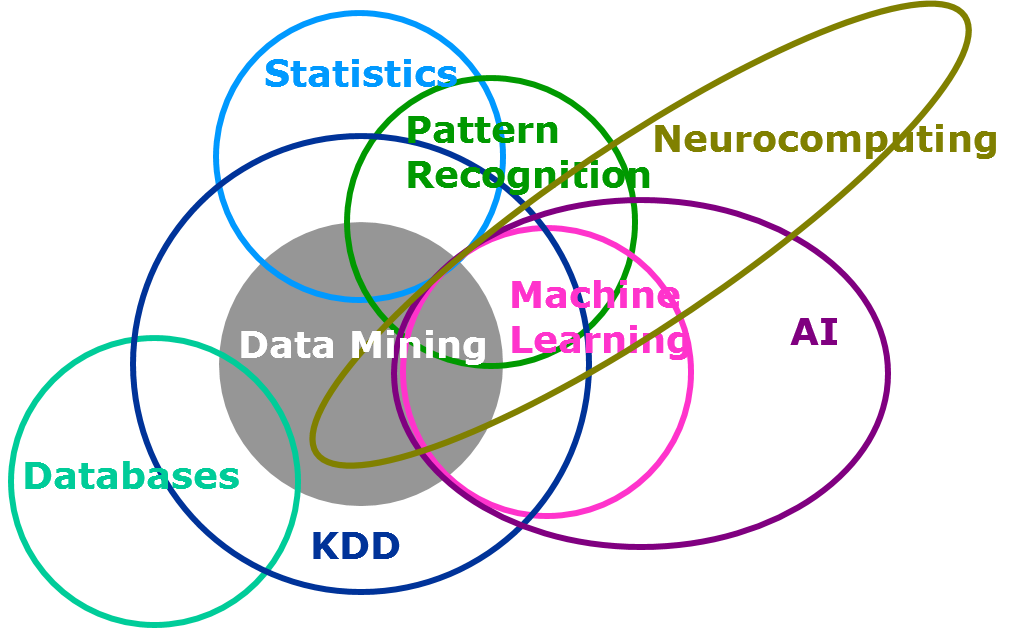
\includegraphics[width=0.75\textwidth]{images/data-mining-venn.png}
\end{center}

\end{frame}

\begin{frame}{Data Mining -- область тысячи имен}

\begin{enumerate}
\item[1960-е] Data Fishing, Data Dredging
\item[1980-е] Knowledge Discovery in Databases
\item[1990-е] Data Mining, Database mining\textsuperscript{TM}
\item[2000-е] Data Analytics, Data Science\footnote{\href{https://twitter.com/nivertech/status/180109930139893761}{Data Scientist is a Data Analyst who lives in California}}\footnote{\href{https://twitter.com/josh_wills/status/198093512149958656}{A data scientist is someone who is better at statistics than any software engineer and better at software engineering than any statistician.}\vspace{1.5em}}
\end{enumerate}

\end{frame}

\begin{frame}{Некоторые важные события в истории Data Mining}

\begin{enumerate}
\item[1989] IJCAI-89 Workshop on Knowledge Discovery in Databases 
\item[1995] ACM SIGKDD Conference on Knowledge Discovery and Data Mining
\item[2001] Leo Breiman's ``Statistical Modeling: The Two Cultures''
\item[2003] Программа Total Information Awareness
\item[2005] Doug Cutting и Mike Cafarella разработали пакет обработки данных Hadoop
\item[2007] Первый релиз библиотки scikit-learn
\item[2010] Заработал сайт Kaggle -- платформа для проведения соревнований по Data Science
\item[2012] Harvard Business Review публикует статью Data Scientist: The Sexiest Job of the 21st Century
\item[2013] Первая встреча сообщества Moscow Data Science\footnote{\url{http://www.meetup.com/Moscow-Data-Science/}\vspace{1.5em}} в московском офисе Mail.Ru Group
\end{enumerate}

\end{frame}

\begin{frame}{CRISP-DM}

(Cross Industry Standard Process for Data Mining)

\begin{center}
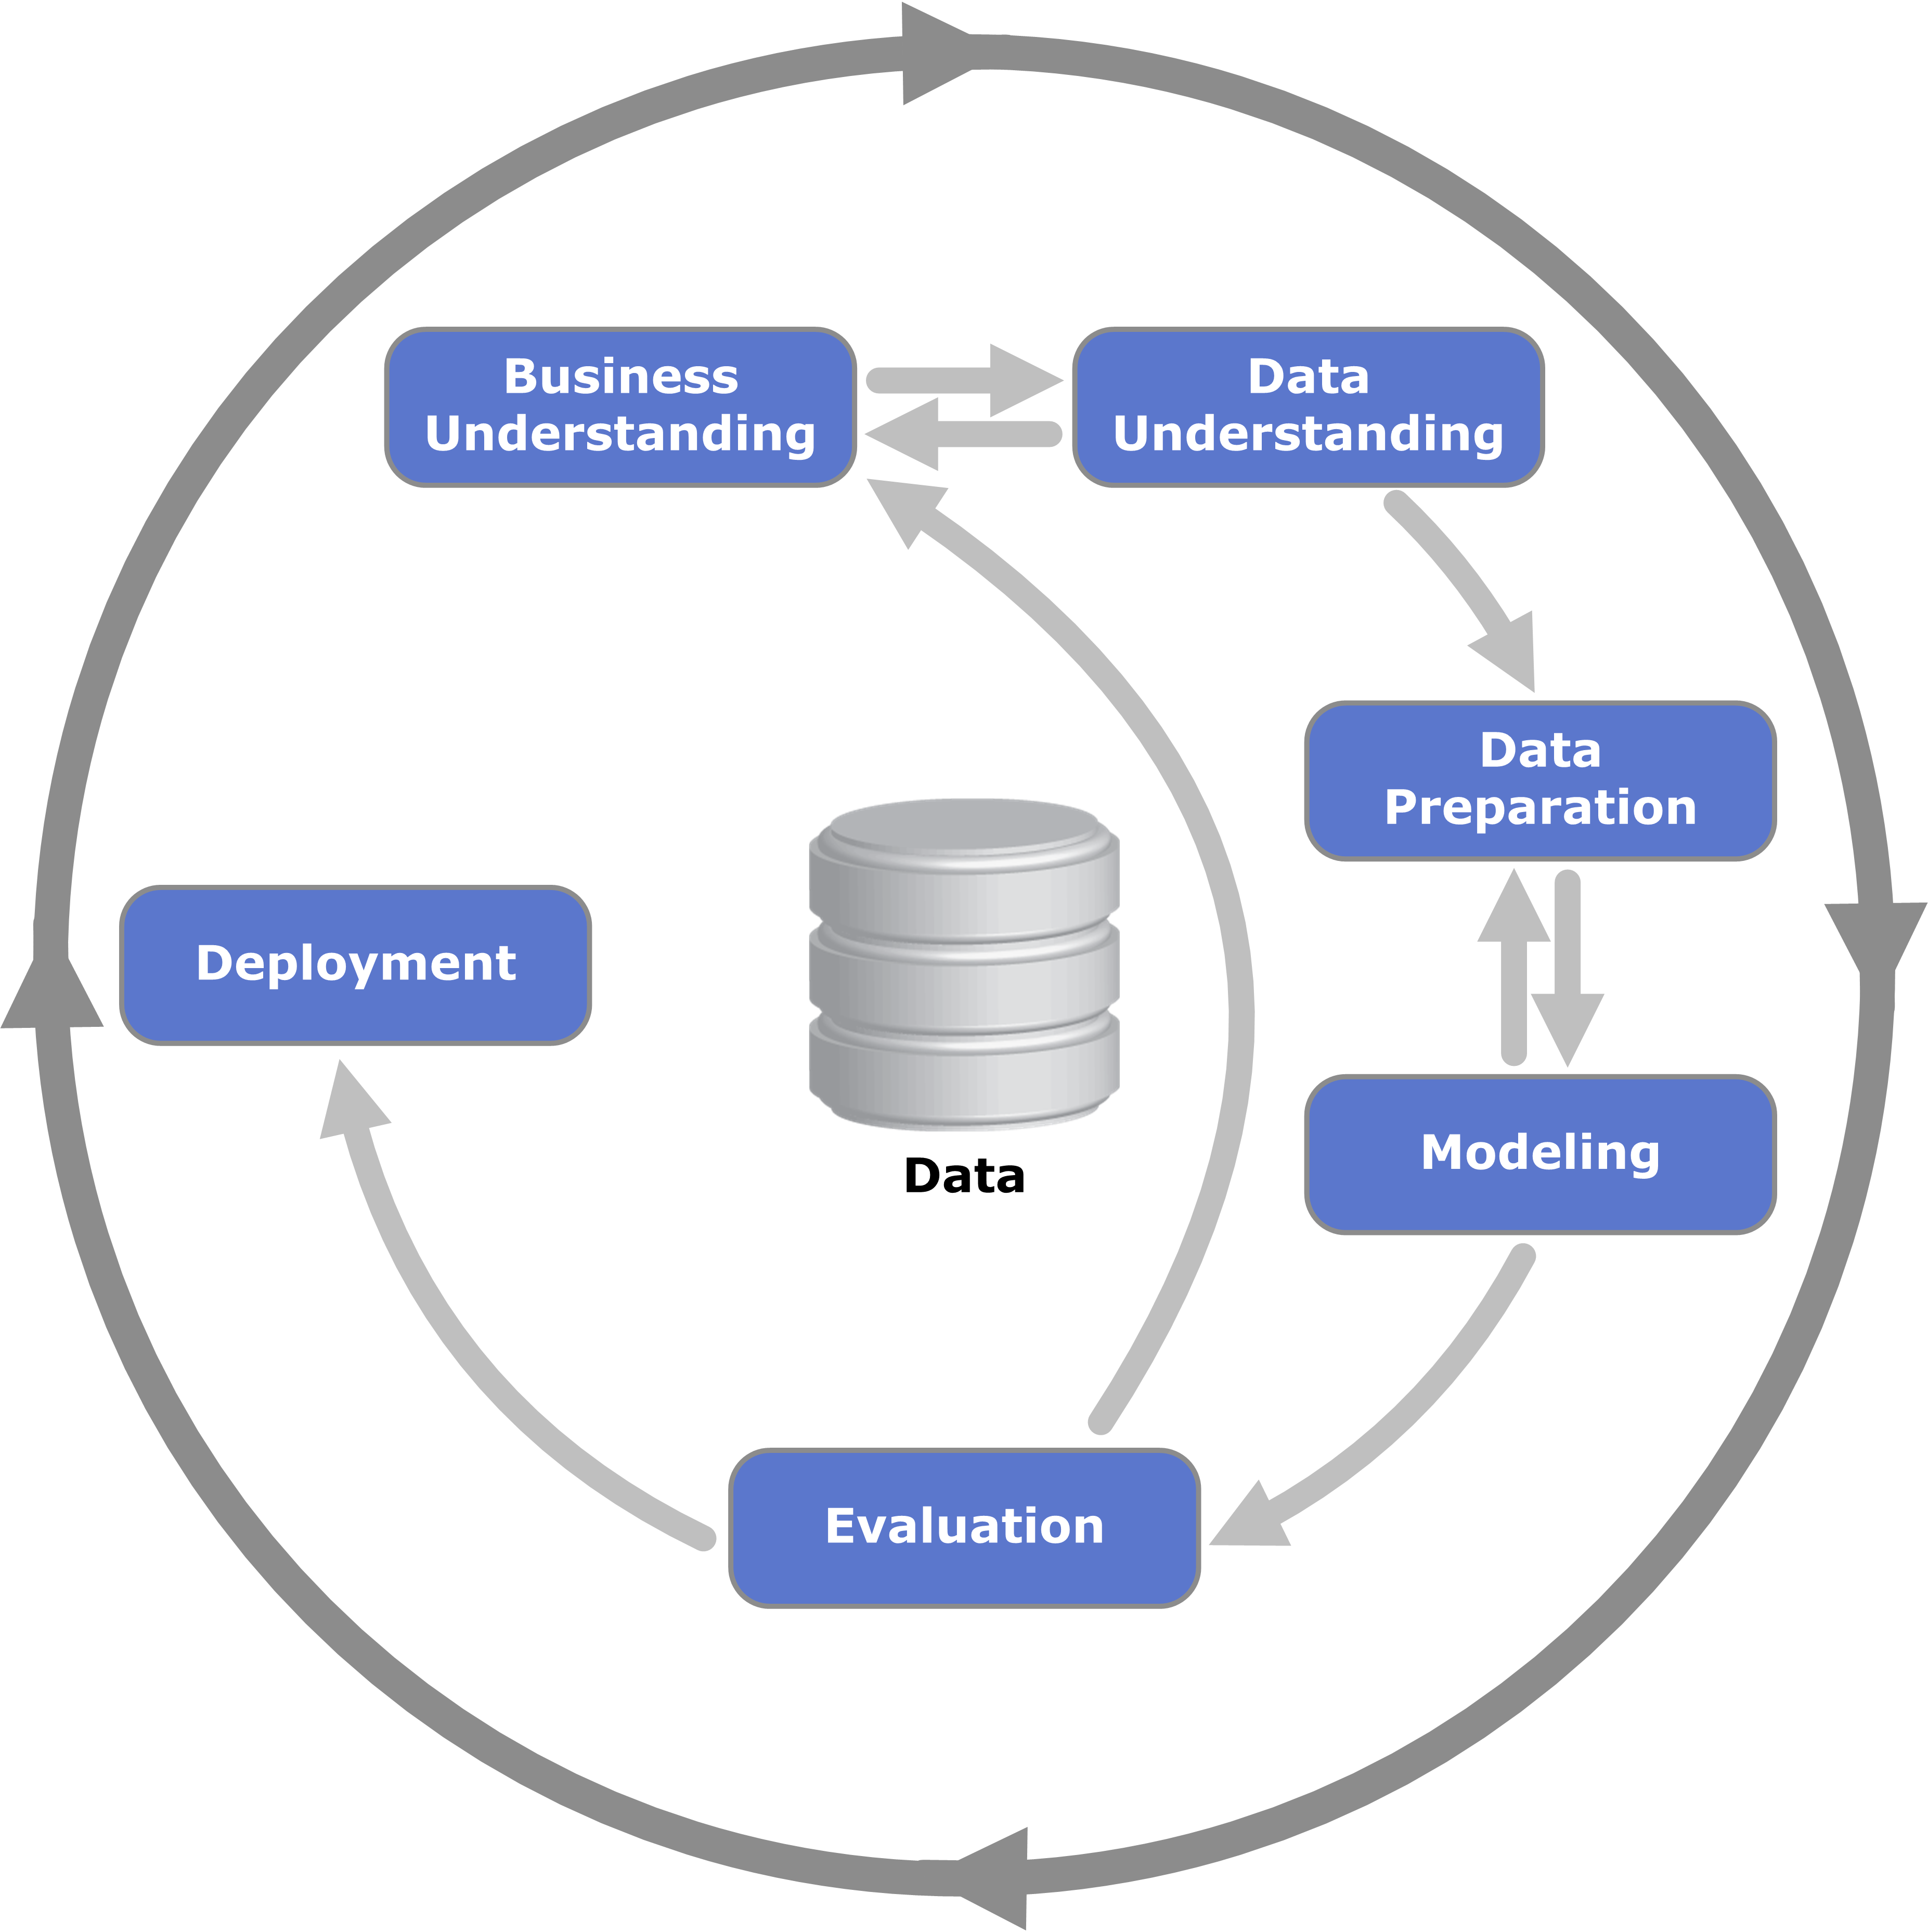
\includegraphics[height=0.7\textheight]{images/crisp.png}
\end{center}

\end{frame}

\begin{frame}{Пример 2. Игра в гольф\footnote{Induction of Decision Trees / R. Quinlan\vspace{1.5em}}}

\begin{columns}
    \begin{column}{.7\textwidth}
    \begin{small}
    	{\bf Business understanding}
		\begin{itemize}
		\item понимание задачи с точки зрения бизнеса
		\item сбор требований и ограничений
		\item постановка задачи в терминах Data Mining
		\end{itemize}
		
		$\mathcal{D}$ -- множество, содержащее все рассматриваемые в задаче объекты \\  \vspace{1em}
		$f: \mathcal{D} \rightarrow \mathcal{Y}$ -- целевая функция \\ \vspace{1em}
		
		Цель -- с использованием данных о конечном множестве объектов из $\mathcal{D}$ (data set) научиться предсказывать значения целевой функции для любых объектов из $\mathcal{D}$
		
		\vspace{1em}
		Задача {\bf с учителем} -- для объектов из data set дано значение целевой функции, иначе -- задача {\bf без учителя}.	
				\end{small}
		
    \end{column}
    %   
    \begin{column}{.3\textwidth}
    \vspace{-0em}
		\begin{center}
   		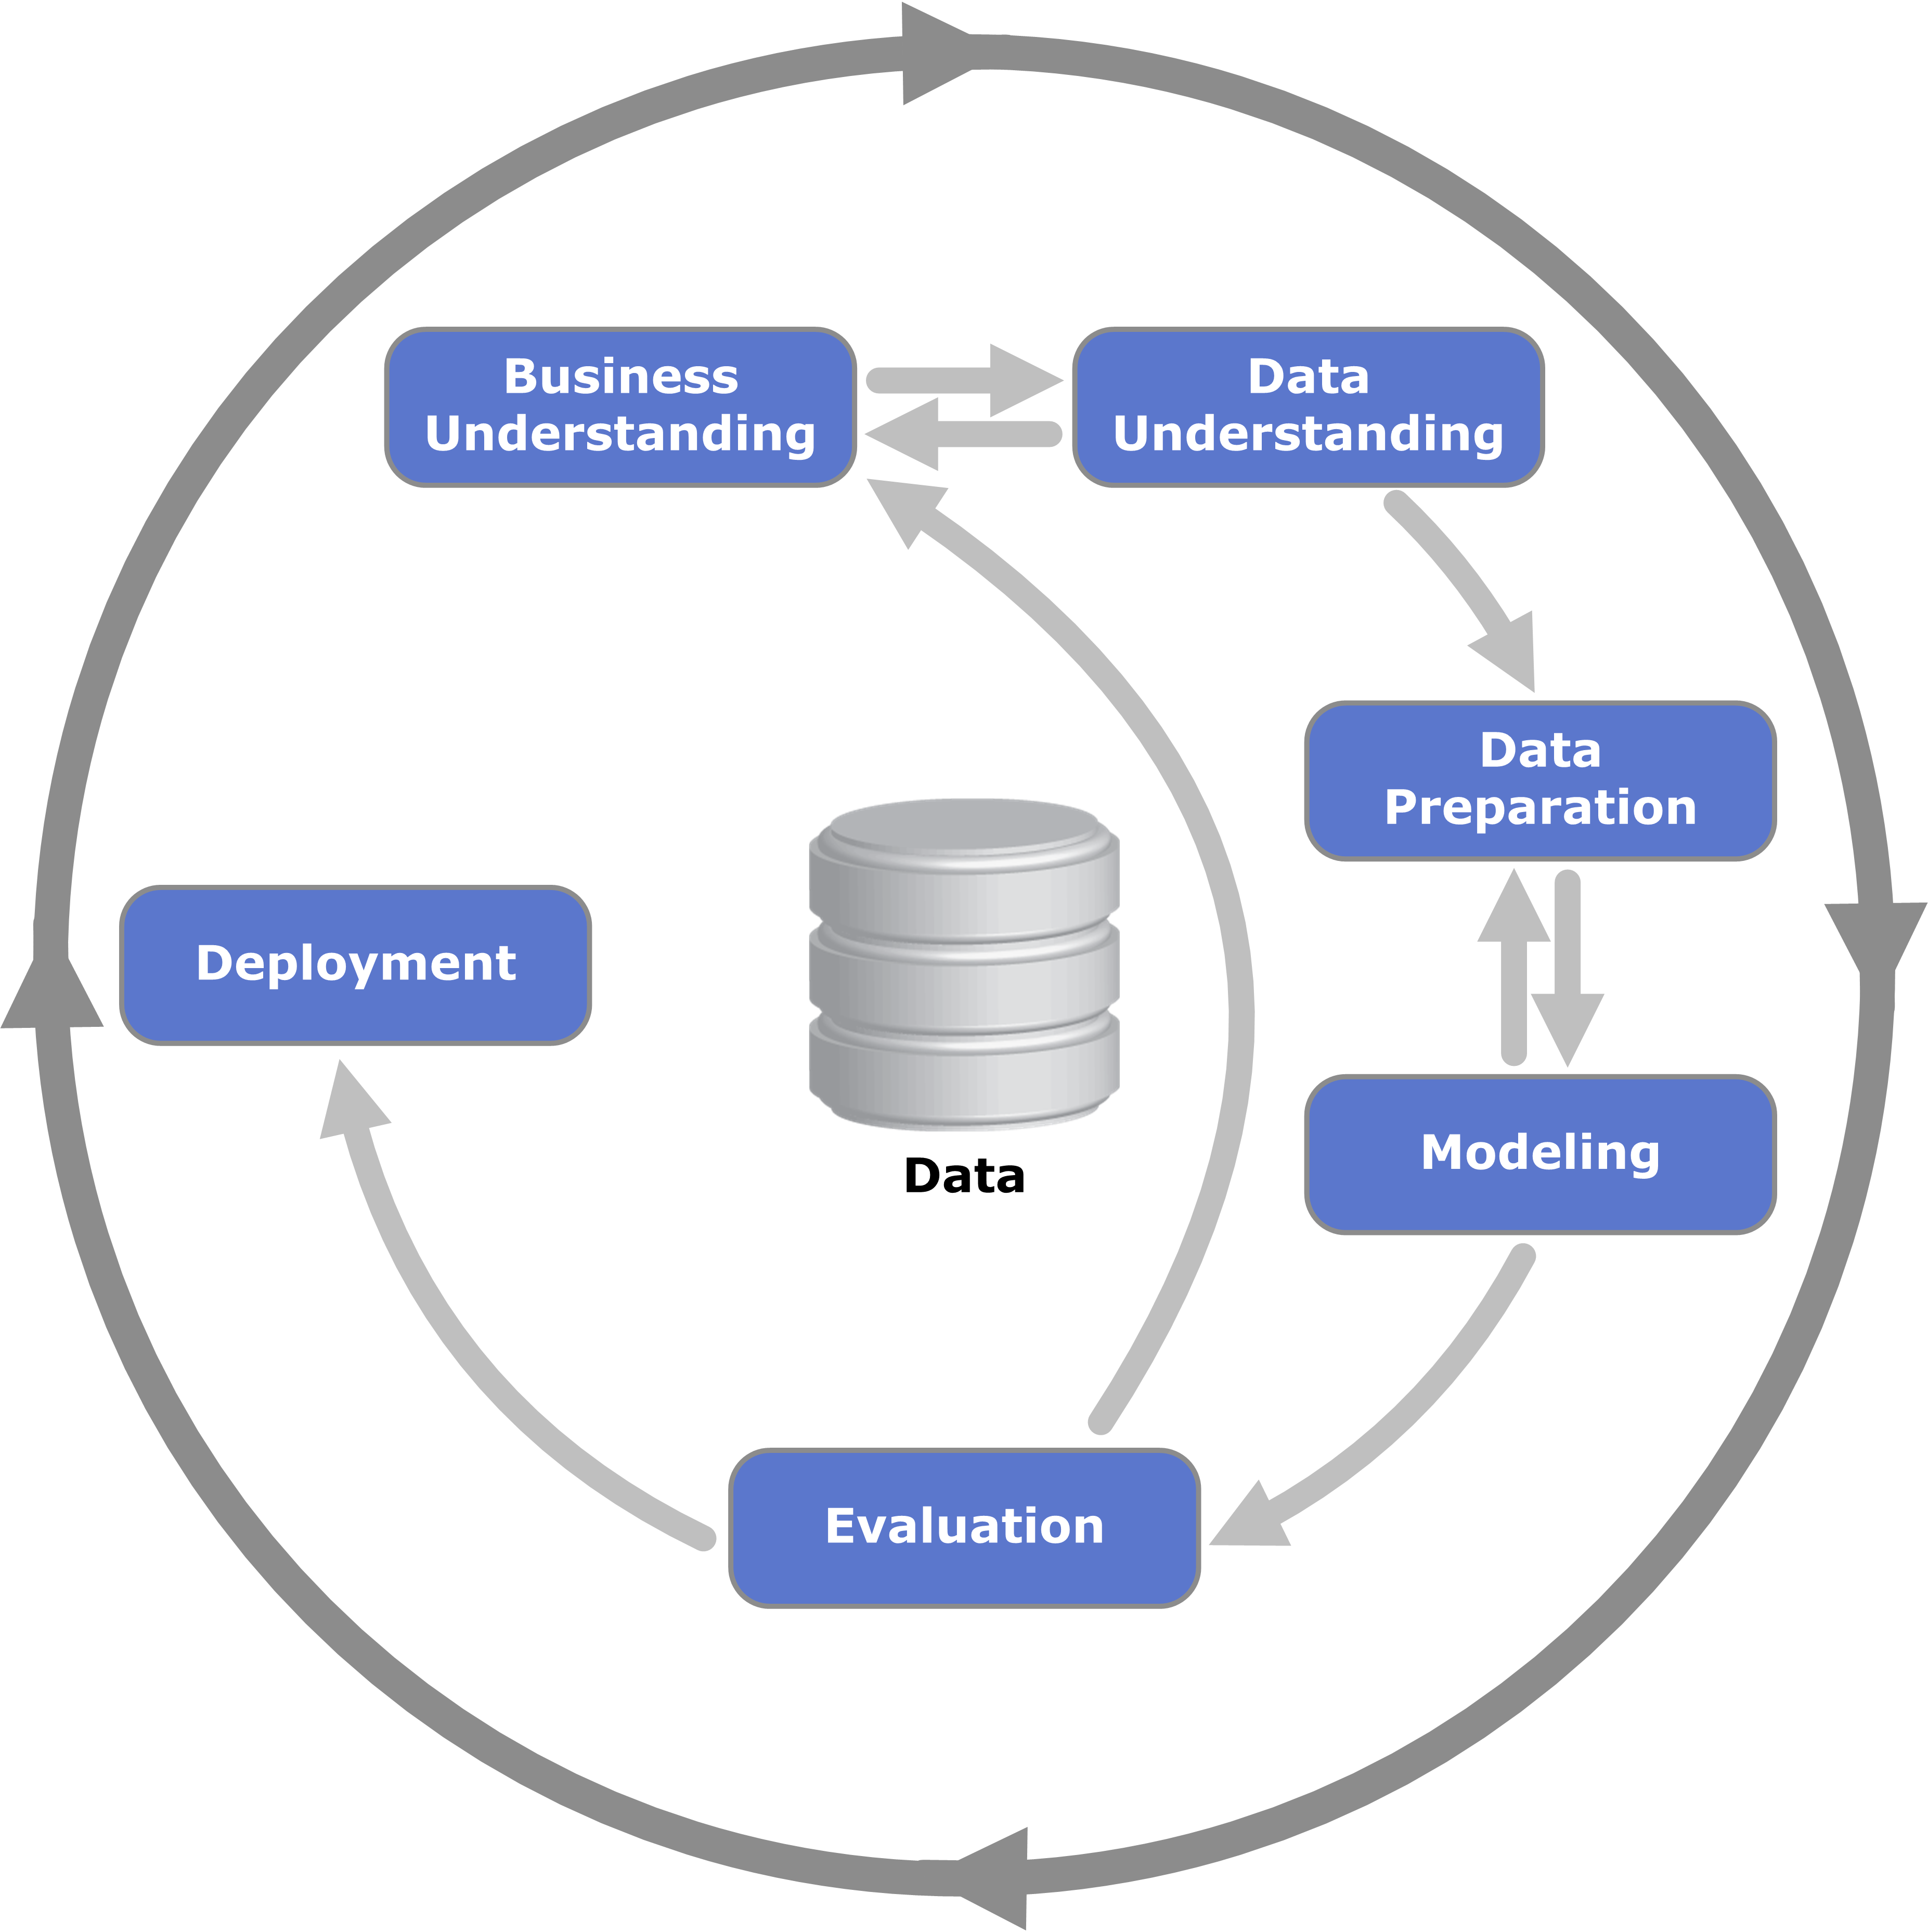
\includegraphics[width=\textwidth]{images/crisp.png}
    \end{center}
    \end{column}
  \end{columns}

\end{frame}

\begin{frame}{Пример 2. Игра в гольф}

\begin{columns}
    \begin{column}{.7\textwidth}
		{\bf Data understanding}
		\begin{itemize}
		\item первичный сбор данных
		\item ознакомление с данными и понимание их специфики
		\end{itemize}
		
		\vspace{1em}

		{\bf Data preparation}
		\begin{itemize}
		\item формирование финального набора данных
		\end{itemize}
    \end{column}
    %   
    \begin{column}{.3\textwidth}
    \vspace{-0em}
		\begin{center}
   		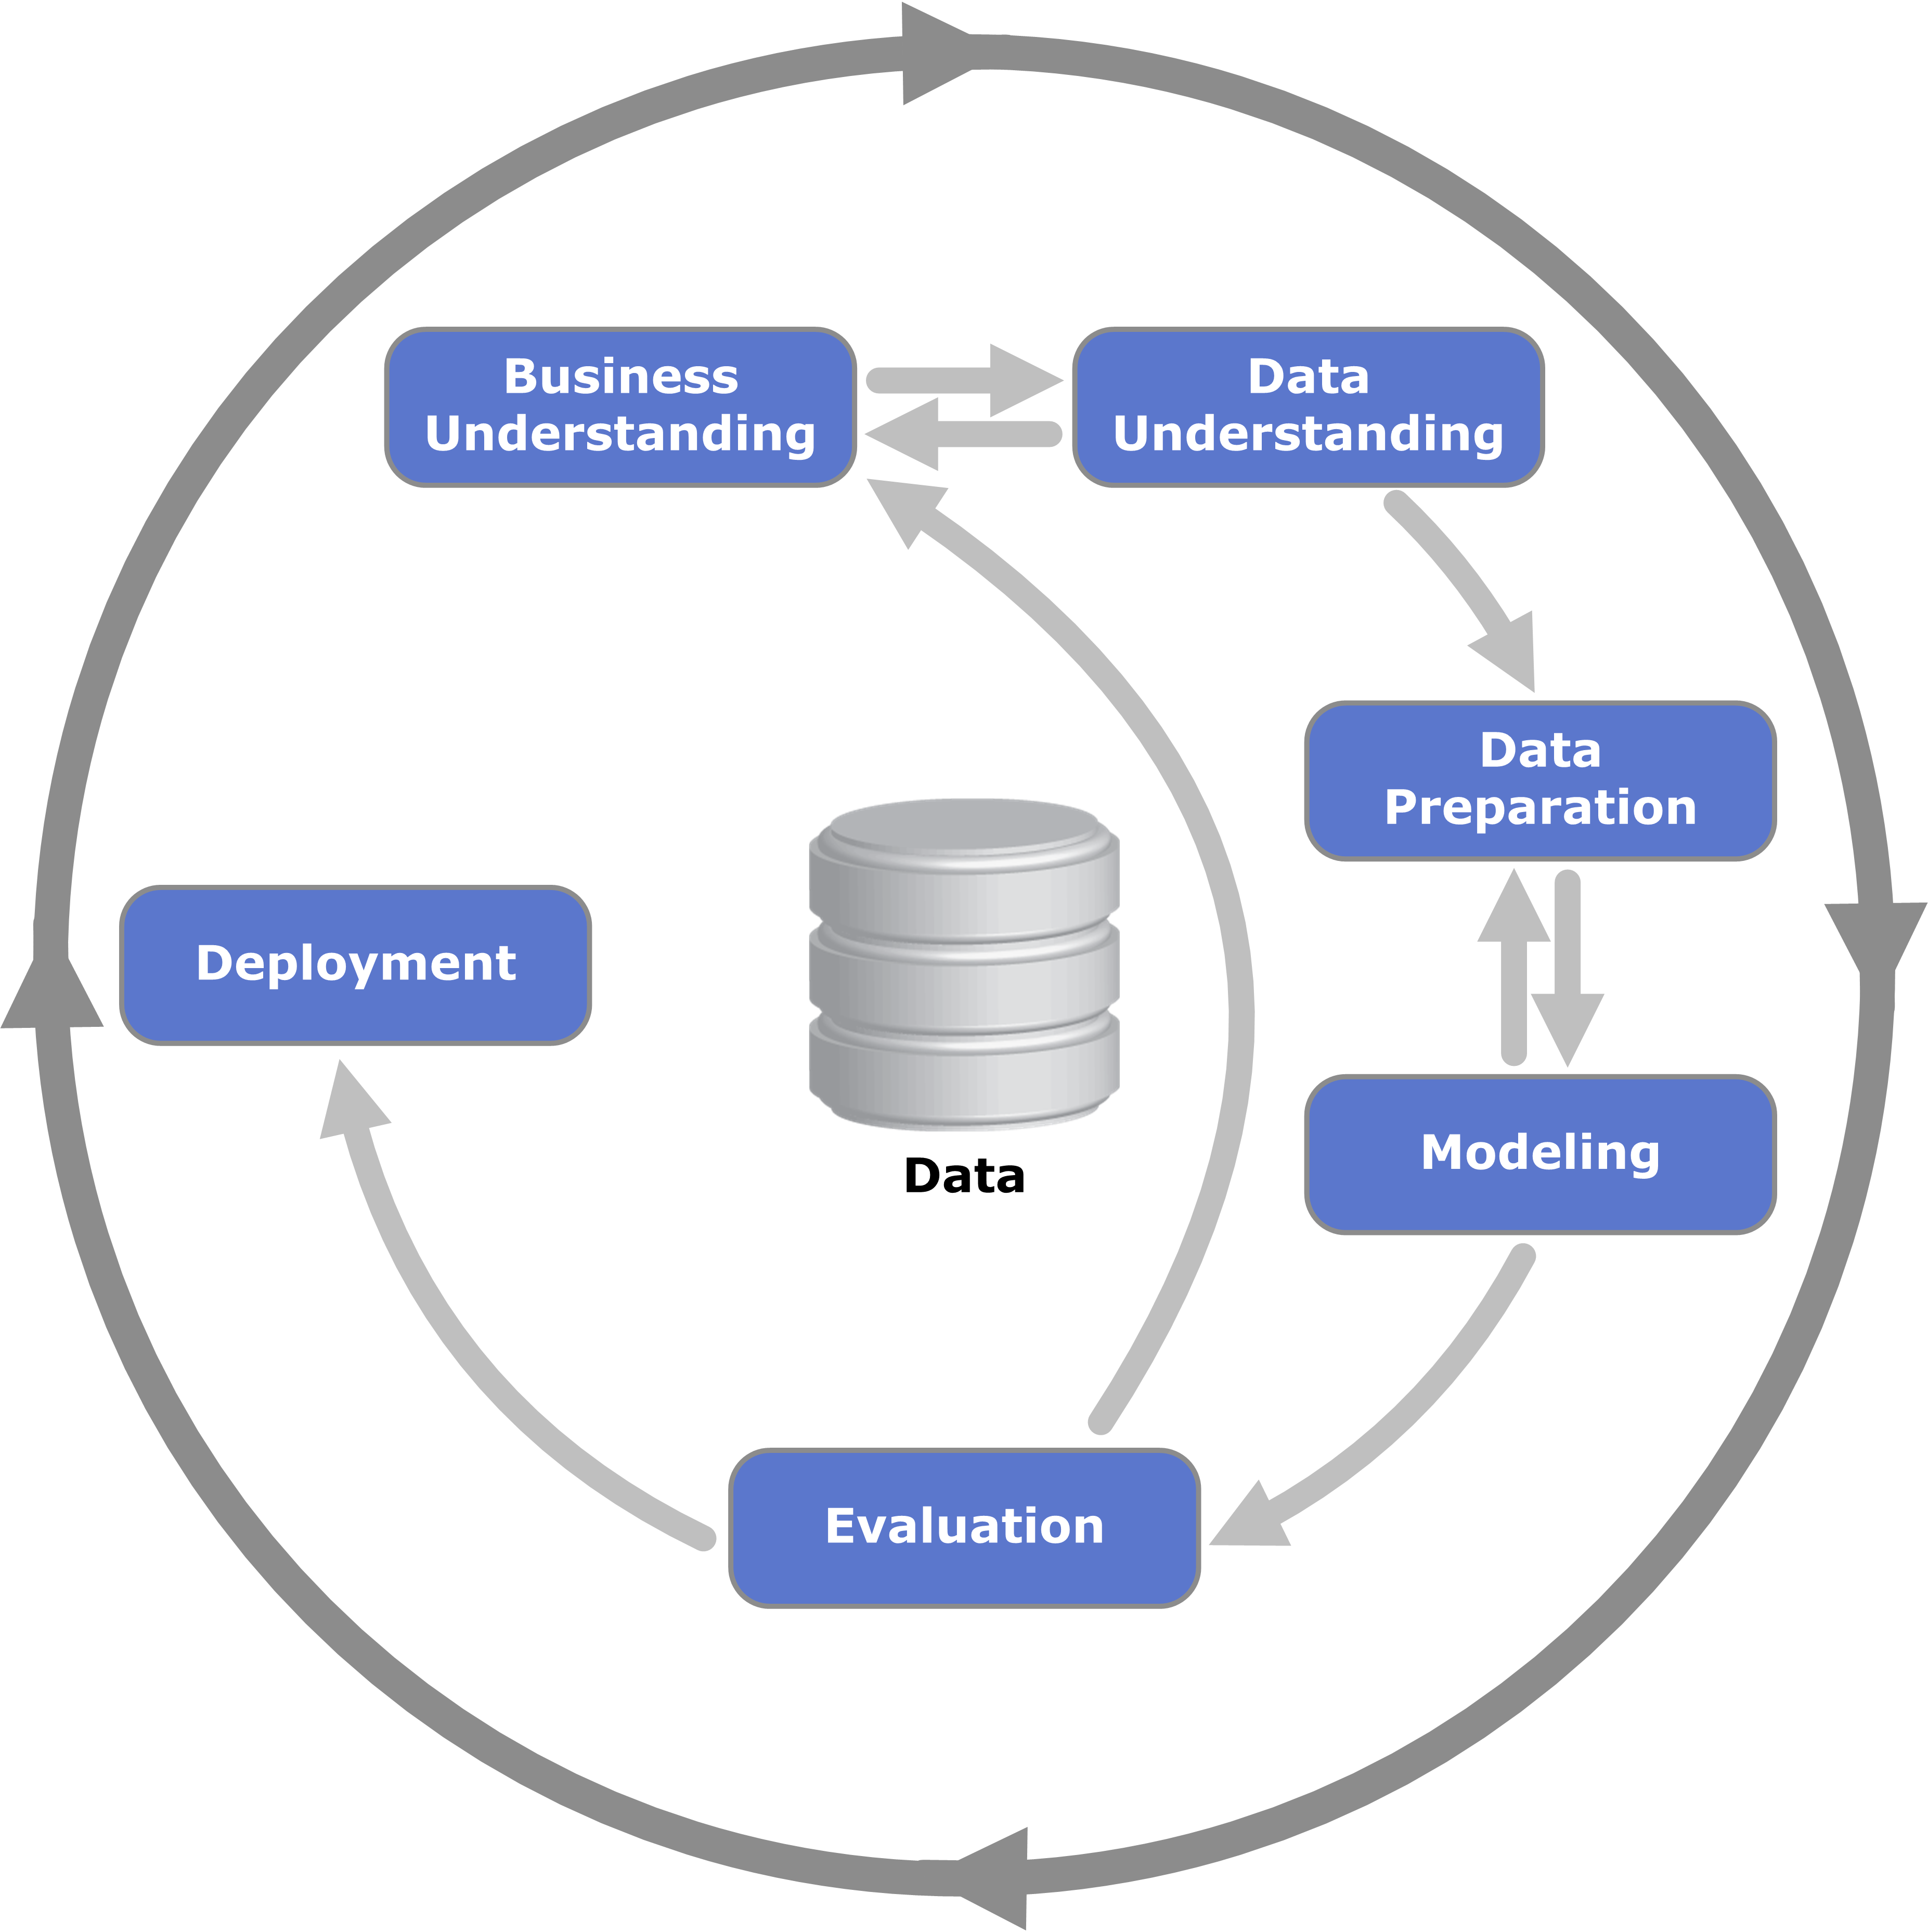
\includegraphics[width=\textwidth]{images/crisp.png}
    \end{center}
    \end{column}
  \end{columns}

\end{frame}

\begin{frame}{Признаки}

$\mathcal{D}$ -- множество, содержащее все рассматриваемые в задаче объекты \\
$d \in \mathcal{D}$ --  объект,  $\phi_j: \mathcal{D} \rightarrow F_j$ -- признак
    
\vspace{1em}
Виды признаков
\begin{itemize}
\item Бинарные/Binary \\ $F_j = \{true, false\}$
\item Номинальные/Categorical \\ $F_j$ -- конечне
\item Порядковые/Ordinal \\ $F_j$ -- конечное, упорядоченное
\item Количественные/Numerical \\ $F_j = \mathbb{R}$
\end{itemize}
\vspace{1em}
Признаковое представление объекта $d$
\[
\mathbf{x} = (\phi_1(d), \ldots, \phi_n(d)) \in \mathcal{X}
\]


\end{frame}

\begin{frame}{Игра в гольф: признаки}

\begin{center}
\begin{tabular}{c | c | c | c | c }
\bf Outlook & \bf Temperature & \bf Humidity & \bf Wind & \bf Play \\
\hline
Sunny & 85 & 85 & false & no \\
Sunny & 80 & 90 & true & no \\
Overcast & 83 & 86 & false & yes \\
Rainy & 70 & 96 & false & yes \\
Rainy & 68 & 80 & false & yes \\
Rainy & 65 & 70 & true & no \\
Overcast & 64 & 65 & true & yes \\
Sunny & 72 & 95 & false & no \\
Sunny & 69 & 70 & false & yes \\
Rainy & 75 & 80 & false & yes \\
Sunny & 75 & 70 & true & yes \\
Overcast & 72 & 90 & true & yes \\
Overcast & 81 & 75 & false & yes \\
Rainy & 71 & 91 & true & no \\
\end{tabular}
\end{center}

\end{frame}

\begin{frame}{Моделирование}

\begin{columns}
\begin{column}{.7\textwidth}
    \begin{itemize}
\item перебор различных моделей
\item настройка параметров моделей
\end{itemize}

\begin{block}{Модель}
признаковое описание объекта $d$:
\[
\mathbf{x} = (\phi_1(d), \ldots, \phi_n(d)) \in \mathcal{X}
\]
значение целевой функции для объекта $d$: $y \in \mathcal{Y}$

\vspace{1em}
{\bf модель} -- семейство функций вида
\begin{empheq}[box=\tcbhighmath]{align}
H = \{h(\mathbf{x}, \theta) \,:\, \mathcal{X} \times \Theta \rightarrow \mathcal{Y} \},\nonumber
\end{empheq}
где $\theta \in \Theta$ -- неизвестный вектор параметров

\end{block}
    \end{column}
    %   
    \begin{column}{.3\textwidth}
    \vspace{-0em}
		\begin{center}
   		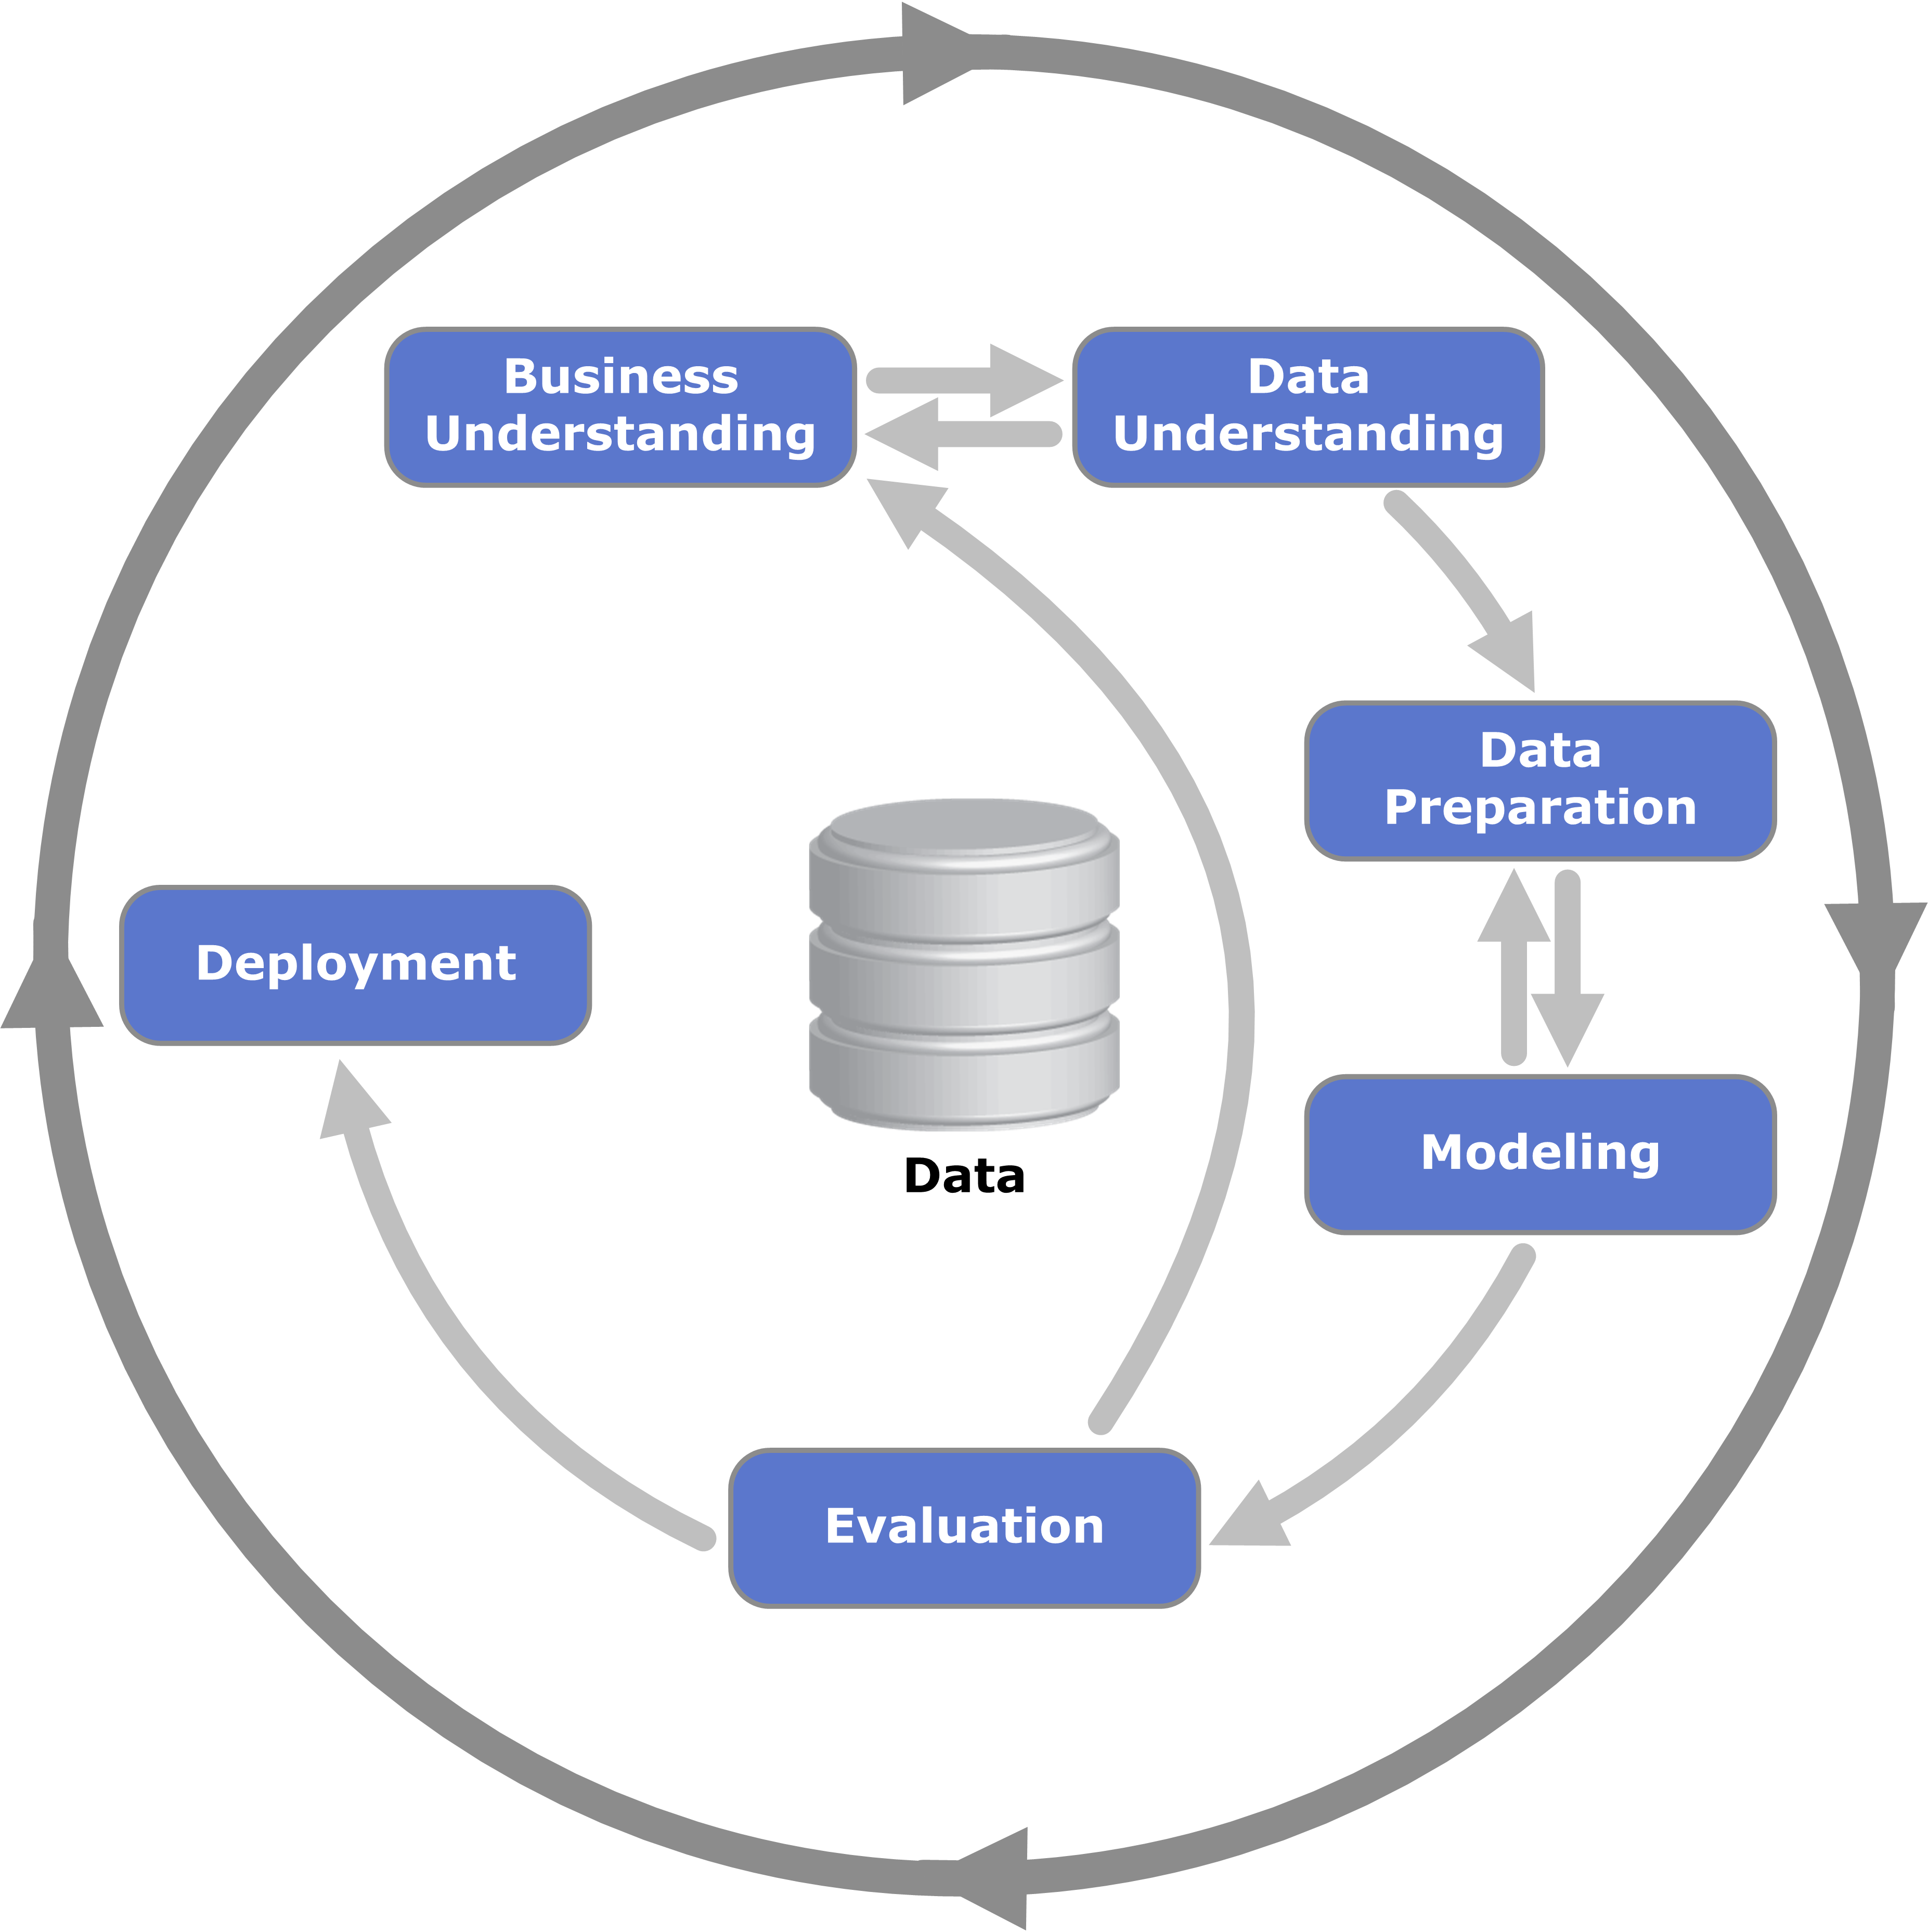
\includegraphics[width=\textwidth]{images/crisp.png}
    \end{center}
    \end{column}
  \end{columns}
    
\end{frame}

\begin{frame}{Пример 1. Снова банки с икрой}
    
{\bf признаковое описание}: $\mathbf{x} \in \mathbb{R}^1$ \\
\vspace{1em}
{\bf целевая переменная}: $y = 1$, если настоящая, $y = 0$ иначе \\
\vspace{1em}
{\bf модель}:
\[
\begin{cases}
p(\mathbf{x} | C_0) \sim \mathcal{N}(\mathbf{x} | \mu_0, \sigma_0), \;\; p(C_0) = \frac 1 2 \\
p(\mathbf{x} | C_1) \sim \mathcal{N}(\mathbf{x} | \mu_1, \sigma_1), \;\; p(C_1) = \frac 1 2
\end{cases} \;\; + \quad y = \mathcal{I}(p(C_1 | \mathbf{x}) > p(C_1 | \mathbf{x}))
\]
\vspace{1em}
{\bf параметры}: $\theta = (\mu_1, \sigma_1, \mu_0, \sigma_0)$

\end{frame}

\begin{frame}{Пример 2. Дерево решений}
    
\begin{columns}
\begin{column}{.5\textwidth}
\begin{center}
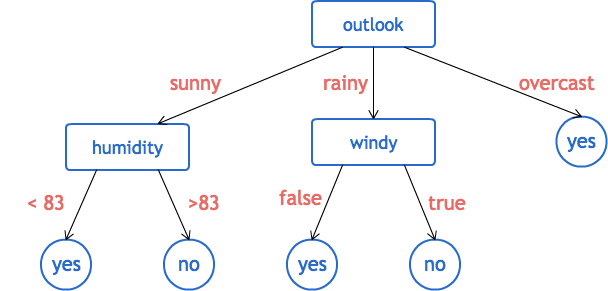
\includegraphics[width=\textwidth]{images/dtree.png}
\end{center}
\end{column}
%   
\begin{column}{.5\textwidth}
\begin{tiny}
\begin{center}
\begin{tabular}{c | c | c | c | c }
\bf Outlook & \bf Temperature & \bf Humidity & \bf Wind & \bf Play \\
\hline
Sunny & 85 & 85 & false & no \\
Sunny & 80 & 90 & true & no \\
Overcast & 83 & 86 & false & yes \\
Rainy & 70 & 96 & false & yes \\
Rainy & 68 & 80 & false & yes \\
Rainy & 65 & 70 & true & no \\
Overcast & 64 & 65 & true & yes \\
Sunny & 72 & 95 & false & no \\
Sunny & 69 & 70 & false & yes \\
Rainy & 75 & 80 & false & yes \\
Sunny & 75 & 70 & true & yes \\
Overcast & 72 & 90 & true & yes \\
Overcast & 81 & 75 & false & yes \\
Rainy & 71 & 91 & true & no \\
\end{tabular}
\end{center}
\end{tiny}
\end{column}
\end{columns}

\end{frame}

\begin{frame}{Обучение модели}

\begin{itemize}
\item дана обучающая выборка (data set) $X = \{{\mathbf{x}_1, \ldots, \mathbf{x_n}}\}$
\item для каждого из объектов обучающей выборки дано значение целевой функции $Y = \{y_1, \ldots, y_n\}$ (если задача с учителем)
\end{itemize}

\begin{block}{Алгоритм обучения}
Выбор наилучших параметров $\theta^*$ с использованием обучающей выборки
\[
A(X, Y): (\mathcal{X} \times \mathcal{Y})^N \rightarrow \Theta
\]
В итоге:
\[
h^*(\mathbf{x}) = h(\mathbf{x}, \theta^*)
\]
\end{block}

\end{frame}

\begin{frame}{Пример 2. Игра в гольф}

\begin{columns}
    \begin{column}{.7\textwidth}
		{\bf Evaluation}
		\begin{itemize}
		\item 
		\end{itemize}
		
		\vspace{1em}

		{\bf Deployment}
		\begin{itemize}
		\item 
		\end{itemize}
    \end{column}
    %   
    \begin{column}{.3\textwidth}
    \vspace{-0em}
		\begin{center}
   		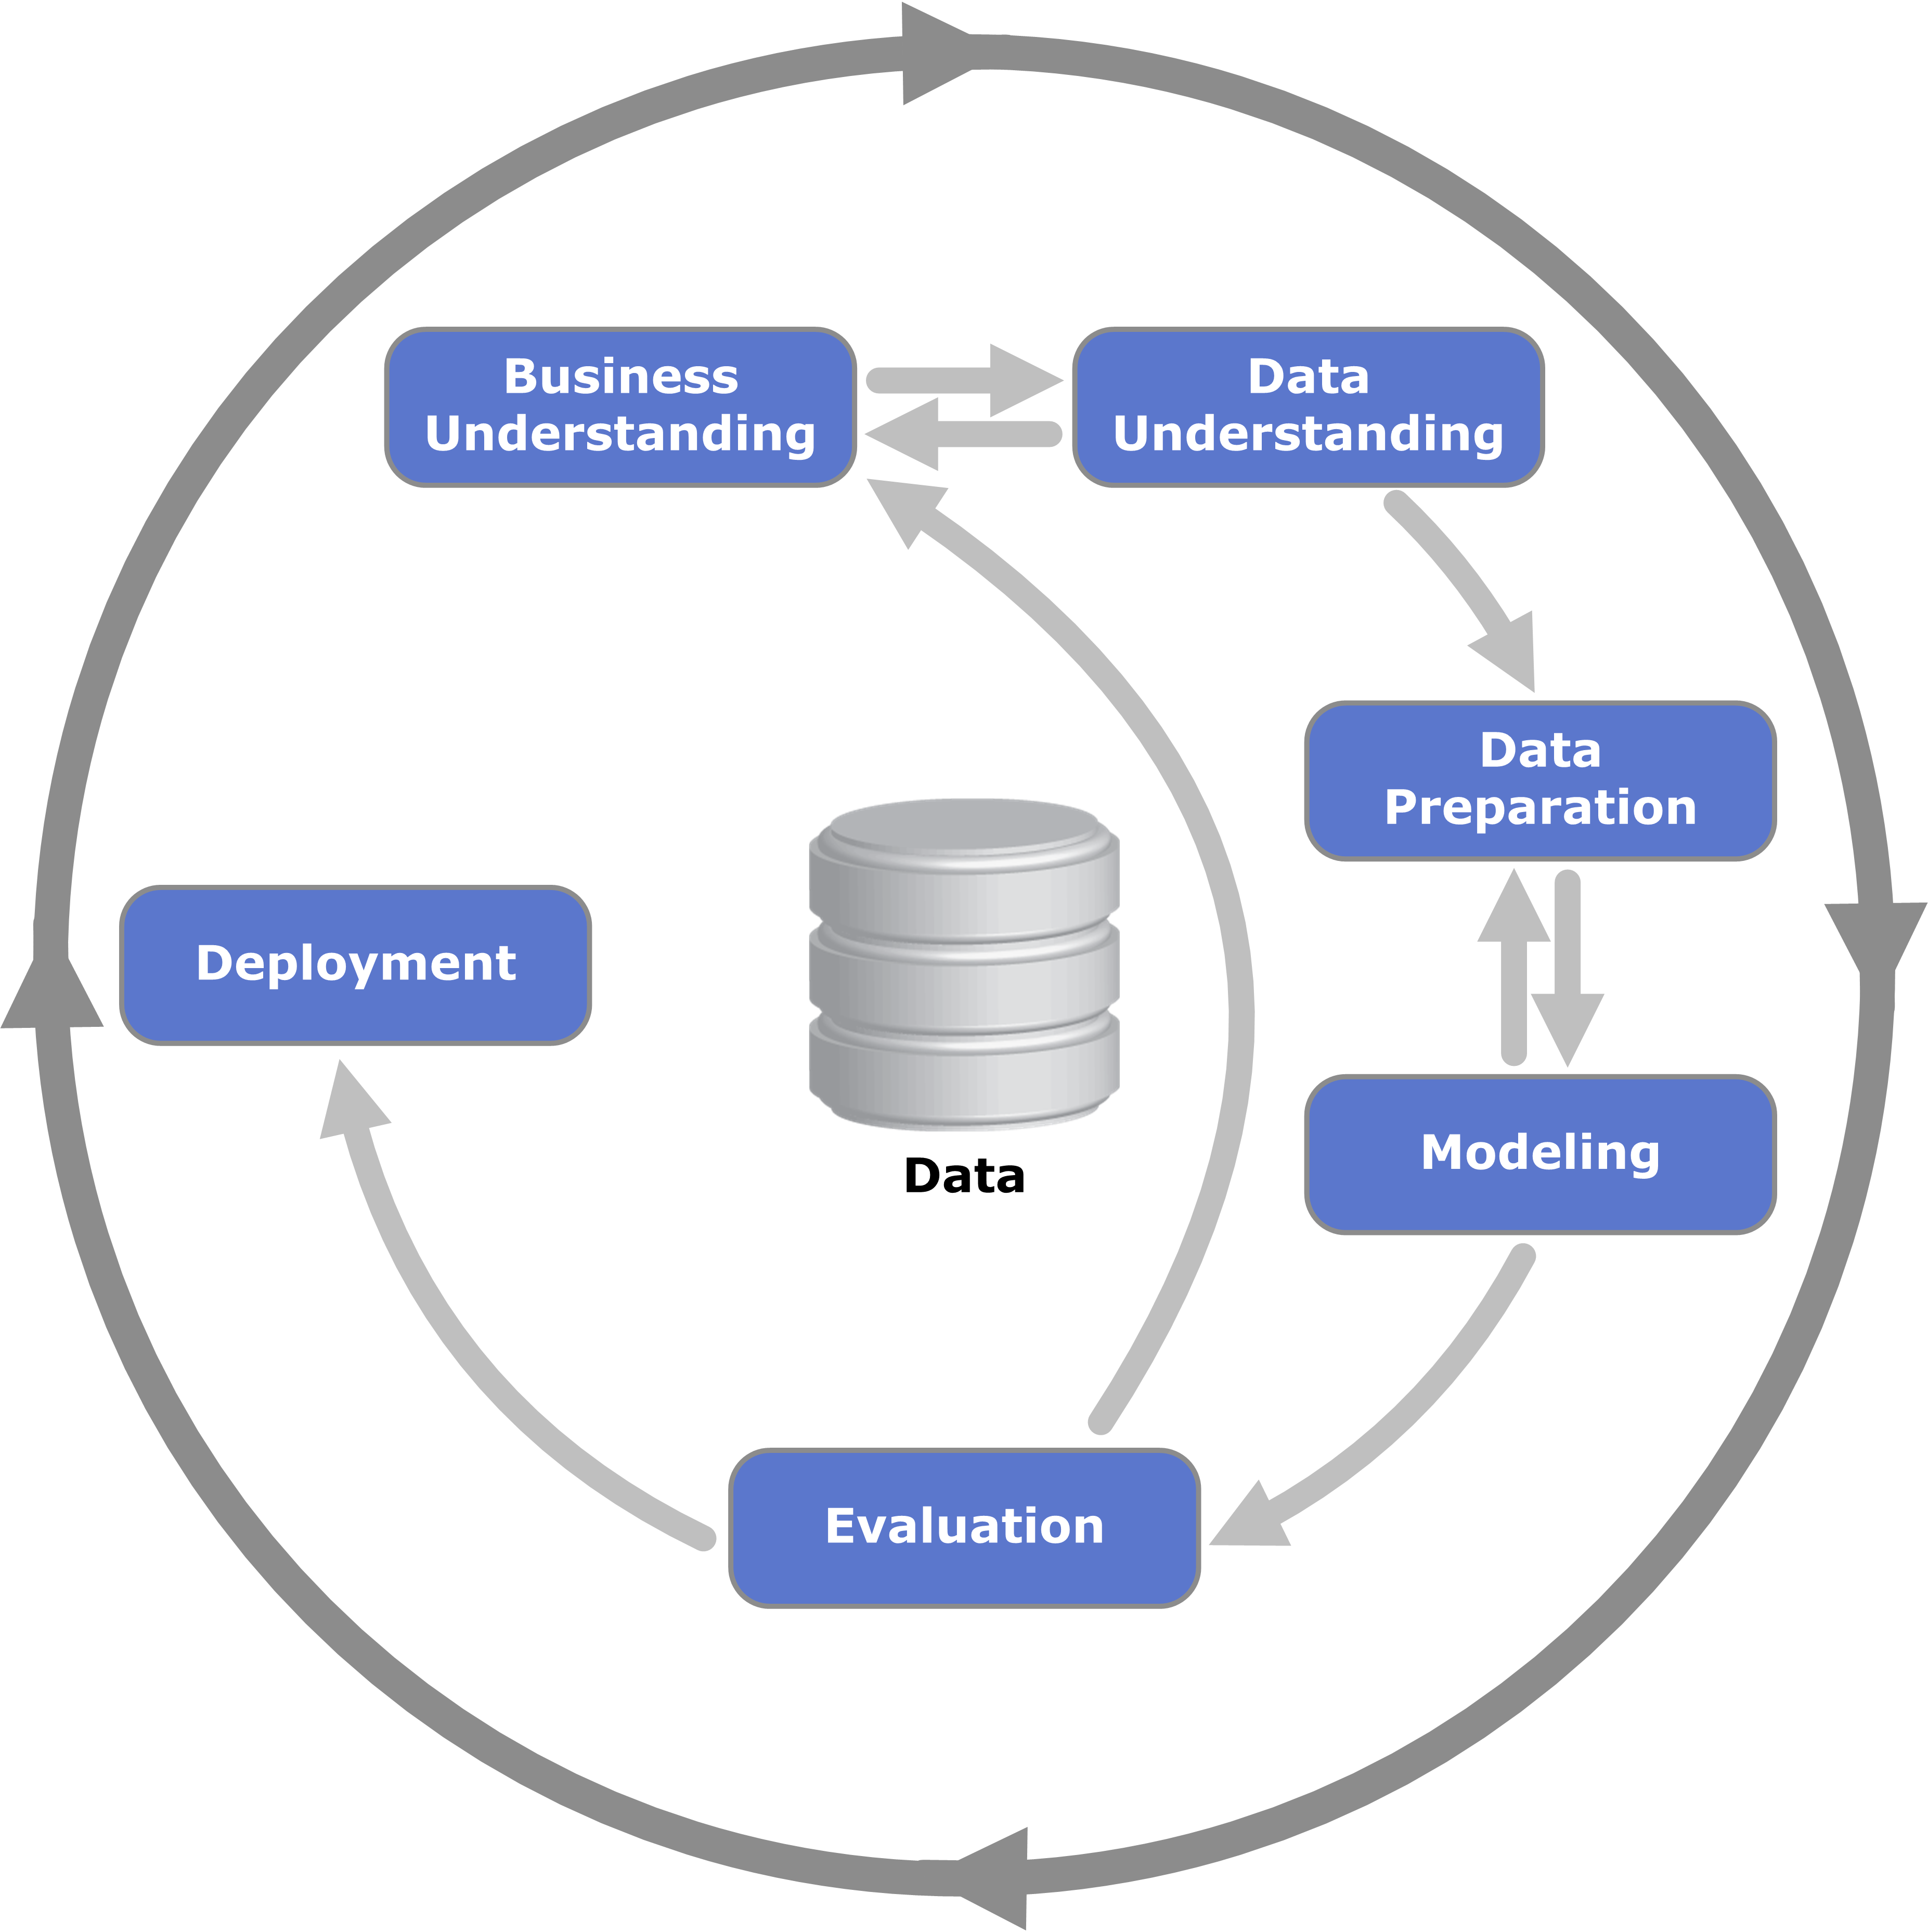
\includegraphics[width=\textwidth]{images/crisp.png}
    \end{center}
    \end{column}
  \end{columns}

\end{frame}


\end{document}